\section{関連研究}
メトリックマップを用いず,
カメラ画像に基づいて自律移動を行う研究はいくつかある.
Dhruvら\cite{shah2022lmnav}は,大規模言語モデル(LLM),視覚言語モデル(VLM),
ビジョンナビゲーションモデル(VLM)の3つの大規模モデルを組み合わせ
自然言語による指示から,画像によるナビゲーションを
end-to-endで行う手法を提案している.

miyamotoら\cite{miyamoto}はランドマークとその接続を含むトポロジカルマップと
カメラ画像のセマンティックセグメンテーションを用いた,走行領域検出による
ビジョンベースのナビゲーション手法を提案している.
\begin{figure}[htbp]
    \centering
     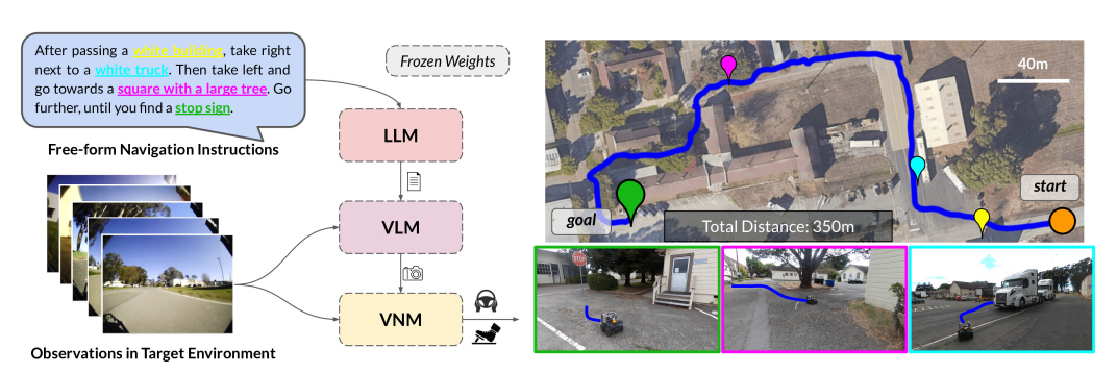
\includegraphics[width=120mm]{images/pdf/lmnav.pdf}
     \caption{Embodied instruction following with LM-Nav Quoted from\cite{shah2022lmnav}}
     \label{fig:lmnav}
\end{figure}

\begin{figure}[h]
    \centering
     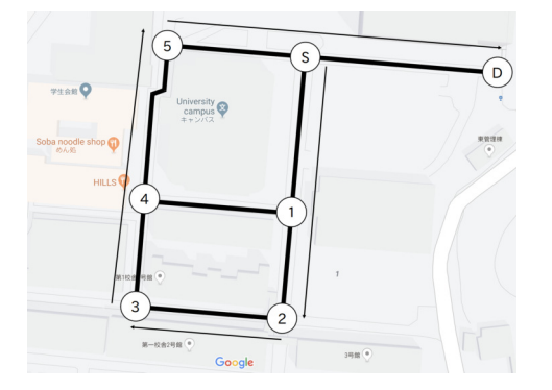
\includegraphics[height=70mm]{images/pdf/topo_meiji.pdf}
     \caption{Topological map Quoted from\cite{miyamoto}}
     \label{fig:topo_meiji}
\end{figure}
\begin{figure}[h]
    \centering
     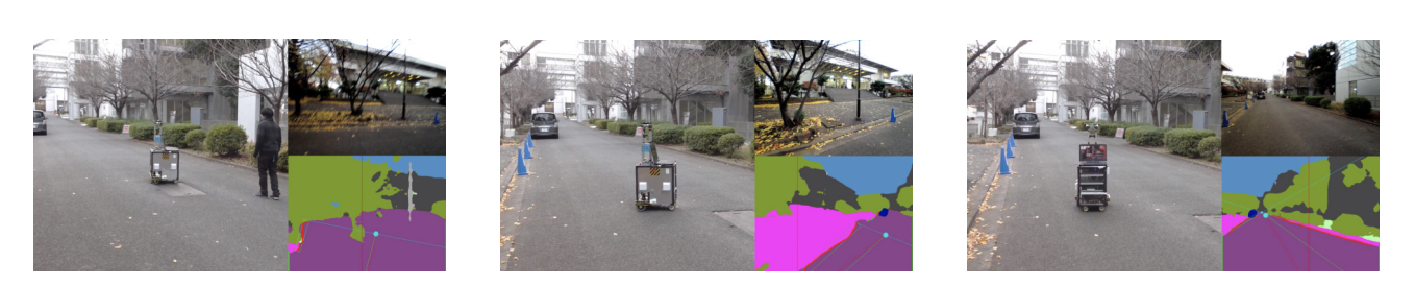
\includegraphics[width=120mm]{images/pdf/seg_meiji.pdf}
     \caption{Observation of robot behavior using semantic segmentation Quoted from\cite{miyamoto}}
     \label{fig:seg_meiji}
\end{figure}

これらの手法では,補助的ではあるが,Global Navigation Satellite System(GNSS)や
ホイールオドメトリといった情報を必要としている.
センサ入力という観点で比較すると,本論文で提案するシステムは
カメラ画像のみで目的地まで移動できるという違いがある.